%Note one sentence in one text line.
\section{Traffic Redirection to Monitor Mobile Internet Traffic} 
\label{sec:platform} 

In this section, we begin by enumerating the goals for practical mobile Internet traffic monitoring.
We then show how \platname extends the existing functionality provided by mobiles OSes and uses traffic redirection to achieve the described goals in a feasible manner. 

\subsection{Goals}  
\label{sec:goals} 
Our primary goal was to obtain comprehensive visibility into the mobile Internet traffic. 
To meet this goal, we further identify the following sub-goals we believe are important to ensure that our approach is practical and feasible. 
\begin{packedenumerate}
\item \emph{Portable.} We want our monitor mobile Internet traffic regardless of operating system, access technology, and service provider of the mobile devices.
Portability ensures that the measurement studies are realisitic and the data collected can be used to compare different OSes, access technologies, and service providers in action.
\item \emph{Pervasive.} Seamless visibility to all the Internet traffic generated by mobile device is essential to ensure that the data collected is comprehensive.
Pervasiveness ensures that the measurement results are realistic and can be used to study real users including those that use mobile devices ``on the move.''
\item \emph{Passive.} The data collected will not comprehensive if traffic monitoring requires explicit triggers from the end users. 
Passiveness also ensures that the system is capable of capture the network traffic even when the devices are \emph{idle}.  
\item \emph{Deployable.} An easy to use and deployable solution that has a low barrier to entry is essential to ensure participation from end users.
\end{packedenumerate}    
In summary, we use portability, pervasiveness, passiveness, and deployablity as the building blocks to define comprehensive and practical monitoring of mobile Internet traffic.  

\subsection{Description}
\label{sec:description}

We posit that traffic redirection can be used to comprehensively monitor mobile Internet traffic.
For our analysis we use two forms of redirection: a VPN based redirection to detail the network traffic characteristics of mobile device, and a transparent proxy based redirection to detail ISP interference of mobile Internet traffic. 

\subsubsection{VPN based Traffic Redirection} 
The use of VPNs by corporate executives ``on the move'' to securely connect to corporate servers with their mobile device was our motivation to consider VPNs.  
VPN usage by corporate clients gave us hints towards the portability and deployability of VPNs.
Further investigation showed us that Mobile OSes expose features that can make them pervasive and suitable for passive monitoring of mobile Internet traffic.  

VPNs are deployable and portable because Android, BlackBerry, Bada, and iOS all support VPNs tunnels over Wi-Fi and the cellular interface.
We now provide an overview of the features that make them pervasive. 
All iOS devices (version 3.0 and above) come with a feature called ``VPN On-Demand''. 
\emph{VPN On-Demand} forces the iOS device to use VPN tunnels when connecting to a specified set of domains. 
Using trial-and-error, we discovered that VPN On-Demand uses suffix matching to determine which domains require a VPN connection. 
We extend this feature to ensure that a VPN tunnel is used when an iOS device connects to the Internet.
Android version 4.0 and above comes with native VPN support. 
Unlike iOS, Android does not offer an equivalent of \emph{VPN On-Demand}; however, Android provides an API that allows an user space app to manage VPN connections. 
We modify the open source StrongSwan VPN client~\cite{strongswanclient} to ensure that the VPN reconnects each time the preferred network changes (\eg, when a device switches from cellular to \wifi). 
As of Android 4.2, Android supports ``Always On'' VPN connections that uses VPNs to tunnel all the data traffic. 
\tbd{Dave:text on Always ON from inputs from Adrian}.

We believe that any practical platform should be based on \emph{off-the-shelf} hardware using open source software. 
Open source VPN solutions to manage VPN tunnels include Strongswan, Openswan, and OpenVPN.
\platname uses Strongswan~\cite{strongswan} because it is the only open source solution that can use the IPsec services of the Linux kernel \emph{without any kernel modifications}.
We emphasize on VPN tunnels created using IPsec, though PPTP and L2TP can be used to create VPNs tunnels, because the \emph{VPN On-Demand} feature of iOS is supported only for VPN tunnels that use IPsec.
Furthermore, Strongswan also supports IKEv2~\cite{rfc5996} protocol used by Android clients and the IKEv1~\cite{rfc4109} protocol used by iOS devices. 
Thus Strongswan, which is used the IPsec services of the Linux kernel ensures that VPN tunnels can be managed using \emph{off-the-shelf} hardware and open source software.

\subsubsection{Redirection using a Transparent Proxy} 

\tbd{Dave add text here} 


\subsubsection{Traffic Monitoring Setup}

\begin{figure}
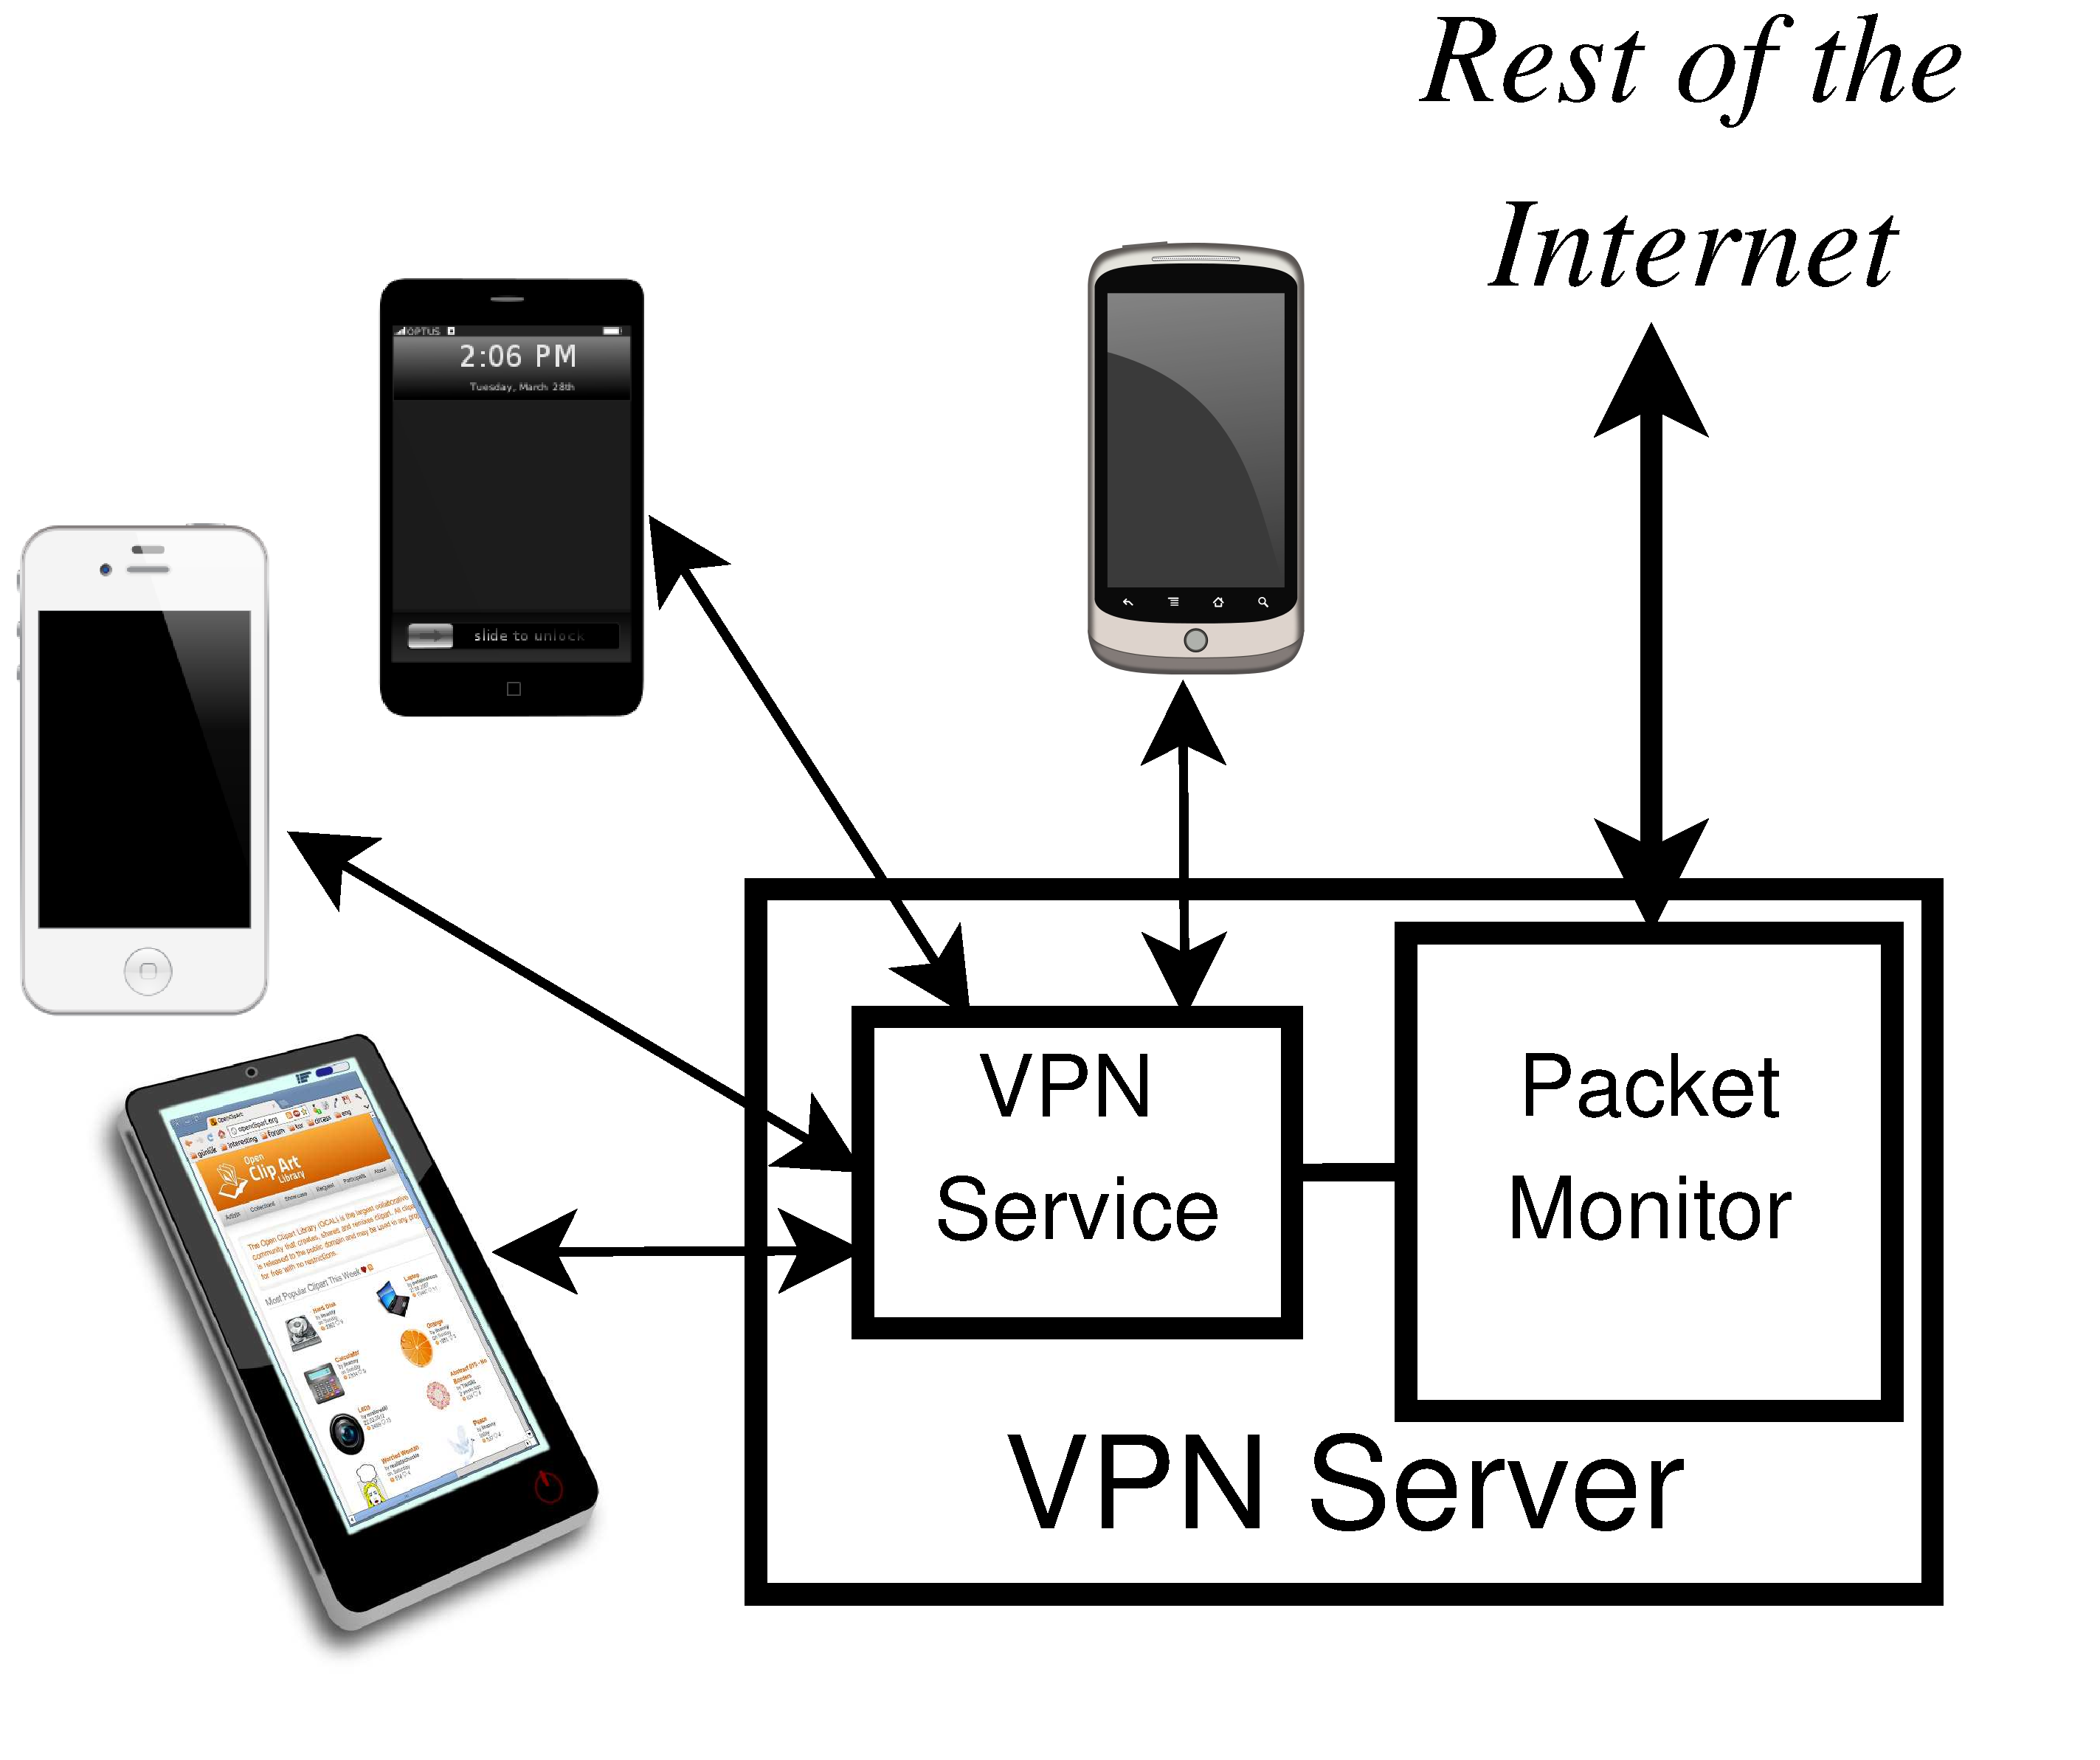
\includegraphics[width=\columnwidth]{figures/meddle-servers.pdf}
\caption{\platname uses traffic redirection to monitor mobile Internet traffic. \platname \emph{requires mobile clients to redirect their traffic through a server that monitors Internet traffic. VPN based redirection is used to characterize mobile traffic sans ISP interference. To detect ISP interference \platname relies on a single hop transparent Web Proxy.}}
\label{fig:description}
\end{figure}

As shown in \fref{fig:description} mobile devices redirect their Internet traffic through a \platname server where all their Internet traffic is monitored. 
\platname uses VPNs for comprehensive monitoring of mobile Internet traffic sans ISP interference.
\platname relies on a a transparent Web proxy to detail interference by mobile ISPs.

Deploying VPNs on mobile clients is simple for end users primarily VPNs are natively supported by popular mobile OSes. 
The Android users need to install a certificate and fill our five fields while iOS users need to install a configuration file. 
Once the configurations are stored, all Internet traffic from the mobile device flows through \platname. 
\platname uses Strongswan to manage VPN tunnels of \platname.
This simplicity is important for practical and realistic measurement studies with end users.

We use tcpdump to monitor the packets that flowing through \platname. 
We now present the technique we used to segregate traffic from mobile devices. 
\platname uses NAT to divert the packets encapsulated in the VPN tunnels to Internet. 
In the ideal scenario, the encapsulated packets from the mobile device would be tunneled to \platname. 
On \platname, these packets would be decapsulated and the packets would then undergo NAT before leaving for their intended destination. 
The packets from the mobile clients to the Internet could be monitored before they undergo NAT.
However, due to the existing network stack implementation, the packets from the Internet that are destined to the mobile clients undergo NAT and IPSec encapsulation take place in one step.
The inter-dependencies between these various modules responsible for routing, NAT, and IPSec make it difficult segregate and monitor the packets. 
We address this issue by looping the packets through a virtual (\emph{tun/tap}) device. 
The looping of packets through a virtual device allows us to monitor the packets when they are outside the VPN tunnels and have not undergone NAT. 

\tbd{Dave: \fref {fig:tripnet} text for tripnet should come here}
\begin{figure}
\centering
\tbd{Dave: New figure for Tripnet comes here.} 
\caption{Overview of the Web tripnet }
\label{fig:tripnet}
\end{figure}


In summary, mobile VPNs are portable and deployable because they are natively supported by popular mobile operating systems.
We build on existing features provided by iOS and Android to make sure that the VPN tunnels are pervasive and are created passively. 
We rely on the open source Strongswan VPN daemon to manage VPN tunnels which makes \platname deployable.
We plan to release the source code to configure mobile Internet traffic using  \platname.

\subsection{Feasibility}

Traffic redirection when using \platname implies that all services that offer features based on IP address of their clients shall react according to the IP address of the server rather than the IP address of the mobile client.
Furthermore, some ISPs are known to block VPNs. 
During our measurement we observed one such ISP that blocked VPN tunnel creation requests from one of our clients.
%Redirection also implies an increase in latency.  
We now show that the cost to redirect traffic in terms of latency, data consumption, and power is sufficiently low.

\subsubsection{VPN Latency Overheads }
The iOS devices use IKEv1 to manage the VPN tunnels while Android devices support both IKEv1 and IKEv2. 
To establish the VPN tunnel, IKEv1 requires a total 16 packets to be exchanged between the mobile client and the VPN server while IKEv2 requires 4 packets.
We use IKEv2 for our Android devices while IKEv1 is used for the iOS devices. 

We performed controlled experiments using one Android device and an iPhone 5 to measure the time required to establish a VPN tunnel. 
We performed this test from two different locations and performed \tbdv{number} of connections over \tbdv{} hours. 
These two locations were based in the same city in which the server was deployed. 
For the Android device, we observe a median connection establishment time of \tbdv{0.62} seconds from both locations when using \wifi with a maximum of \tbdv{0.81} seconds. 
The median connection establishment time was \tbdv{0.81} seconds with a maximum of \tbdv{1.59} seconds from both locations when the Android device used cellular networks to establish the tunnel.
Compared to the Android device, the iOS devices required a larger amount of time to establish the connection. 
We observed a median connection establishment time of \tbdv{1.60} seconds and \tbdv{1.34} seconds with a maximum of \tbdv{2.0} seconds and \tbdv{1.48} seconds respectively from the two Wi-Fi networks; in the case of cellular networks  we observed a median of \tbdv{1.80} seconds and \tbdv{1.65} seconds with a maximum of \tbdv{2.18} seconds and \tbdv{1.87} seconds respectively. 

In summary, we observe that because iOS devices take up to twice as much time as Android devices because iOS devices use an older key management algorithm (IKEv1). \tbd{Any more insights .. The tunnel establishment times in the order of 2 seconds implies that \platname can have a significant latency overhead if VPN tunnels are established periodically for short tests.}

\subsubsection{Data Consumption Increase when using VPN}
IPSec encapsulation slightly inflates packet sizes, in addition to preventing carrier middleboxes from applying their own compression.
We measured the overhead of the tunnel in terms of data overhead from IPsec headers and keep-alive messages, finding that it
ranges from \tbdv{8--12.8}\%.

For our measurements, we capture the encrypted packets exchanged by our \platname servers and the mobile clients that use \platname. 
We performed the packet capture for \tbdv{30} days during which \tbdv{25} devices tunneled their traffic via  \platname. 
During this time interval we also capture the packets that were encapsulated in the IPsec packets. 
We use these samples to compute the increase in the amount of bytes transferred due to encapsulation and the keep-alive
messages. 
During the \tbdv{30} day period we observe that the median of the increase to be \tbdv{8.31\%}, with a maximum increase of \tbdv{12.8\%}.

\tbd{In summary, we observe a maximum overhead of 12.8\% increase in data consumption. We believe the costs of this overhead are minimal compared to the cost of warrant voiding the device.}

\subsubsection{Power Overheads when using VPNs}
\tbd{Daves results}

\tbd{In summary, we show \platname is feasible to build and deploy}

\subsubsection{Impact of using Transparent Proxy}

\tbd{Dave: Text comes here}

\subsection{Discussion}

In this section we show that traffic redirection can be used for comprehensive monitoring of mobile Internet traffic.
\platname relies on the low barrier to entry offered by VPNs that can be served using \emph{off-the-shelf} hardware and open source software. 
\tbd{some more text here on the pros and cons of this approach}
We now show how we used \platname for measurements using real users and also for  controlled experiments to detail the characteristics of mobile Internet traffic. 




